\documentclass[11pt,a4paper,spanish]{book}  % book, article

\usepackage[english]{babel}
\usepackage[utf8]{inputenc}
% Paquetes para incluir graficos:
\usepackage{graphics}
\usepackage{graphicx}
\usepackage{epstopdf}
% Tratamiento de graficos
\usepackage{picture}
% Colores
\usepackage[usenames]{color}
% Texto preformateado
\usepackage{verbatim}
\usepackage{listings}
% Hipervinculos (indice y URLs)
\usepackage{hyperref}
% Matematicas
\usepackage{amsfonts}
\usepackage{amsmath}
\usepackage{amsthm}
\usepackage{amssymb}
\usepackage{anysize}
\usepackage{caption}
\usepackage{geometry}
\usepackage[final]{pdfpages}
\usepackage{cite}
\usepackage{natbib}
\usepackage[numbib,notlof,notlot,nottoc]{tocbibind}

\newcommand{\HRule}{\rule{\linewidth}{0.5mm}}

%%PER EL CODI EN C%%%
\usepackage{listings}
\lstset{ %
language=C++,                % choose the language of the code
basicstyle=\footnotesize,       % the size of the fonts that are used for the code
numbers=left,                   % where to put the line-numbers
numberstyle=\footnotesize,      % the size of the fonts that are used for the line-numbers
stepnumber=1,                   % the step between two line-numbers. If it is 1 each line will be numbered
numbersep=5pt,                  % how far the line-numbers are from the code
backgroundcolor=\color{white},  % choose the background color. You must add \usepackage{color}
showspaces=false,               % show spaces adding particular underscores
showstringspaces=false,         % underline spaces within strings
showtabs=false,                 % show tabs within strings adding particular underscores
frame=single,           % adds a frame around the code
tabsize=2,          % sets default tabsize to 2 spaces
captionpos=b,           % sets the caption-position to bottom
breaklines=true,        % sets automatic line breaking
breakatwhitespace=false,    % sets if automatic breaks should only happen at whitespace
escapeinside={\%*}{*)}          % if you want to add a comment within your code
}

%%%%%%%% Entornos teorema, definiciÛn, comentario, ... %%%%%%%%
\swapnumbers  % Poner el numero del teorema ANTES del teorema.

\theoremstyle{definition}  % Titulo en negrita y texto plano

\newtheorem{definicion}{Definicion}[chapter]
\newtheorem{ejemplo}[definicion]{Ejemplo}
\newtheorem{comentario}[definicion]{Comentario}
\newtheorem{propiedades}[definicion]{Propiedades}
\newtheorem*{objetivo}{Objetivo}
\newtheorem*{idea}{Idea}

\theoremstyle{plain}  % Titulo en negrita y texto en cursiva.
\newtheorem{teorema}[definicion]{Teorema}
\newtheorem{proposicion}[definicion]{ProposiciÛn}
\newtheorem{corolario}[definicion]{Corolario}
\newtheorem{lema}[definicion]{Lema}

\theoremstyle{remark}  % Titulo en cursiva y texto plano
\newtheorem*{observacion}{ObservaciÛn}
\newtheorem*{ejercicio}{Ejercicio propuesto}
\newtheorem*{pregunta}{Pregunta}

%%%%%%%% Formato cÛdigo incluido %%%%%%%% 
\lstset{ %
%language=Octave,                % choose the language of the code
basicstyle=\footnotesize,       % the size of the fonts that are used for the code
numbers=left,                   % where to put the line-numbers
numberstyle=\footnotesize,      % the size of the fonts that are used for the line-numbers
stepnumber=1,                   % the step between two line-numbers. If it's 1 each line 
                                % will be numbered
numbersep=5pt,                  % how far the line-numbers are from the code
%backgroundcolor=\color[rgb]{0.8,0.8,0.8},  % choose the background color. You must add \usepackage{color}
showspaces=false,               % show spaces adding particular underscores
showstringspaces=false,         % underline spaces within strings
showtabs=false,                 % show tabs within strings adding particular underscores
frame=single,	                % adds a frame around the code
tabsize=2,	                % sets default tabsize to 2 spaces
captionpos=b,                   % sets the caption-position to bottom
breaklines=true,                % sets automatic line breaking
breakatwhitespace=false,        % sets if automatic breaks should only happen at whitespace
title=\lstname,                 % show the filename of files included with \lstinputlisting;
                                % also try caption instead of title
escapeinside={\%*}{*)},         % if you want to add a comment within your code
morekeywords={*,...}            % if you want to add more keywords to the set
}




%\marginsize{3 cm}{2 cm}{2 cm}{2.5 cm}

%\title{\textbf{Project Handbook for Development Projects}}
%\author{Carolina Millet \\ Xavier Bush}
%\date{October 2014}		% Comentar para que aparezca la fecha de hoy
\newgeometry{
    top=35mm,
    bottom=30mm,
    outer=30mm,
    inner=30mm,
}

\begin{document}


\begin{titlepage}
\begin{center}


\textsc{\LARGE Kungliga Tekniska Högskolan}\\[1.5cm]

\textsc{\Large ~}\\[-0.5cm]


{ \huge \bfseries \textbf{Project Report} \\

\HRule

 Noise and echo cancellation in a teleconference\\[0.4cm]}

\HRule \\[1.1cm]

		\begin{figure}[h]
		\centering
		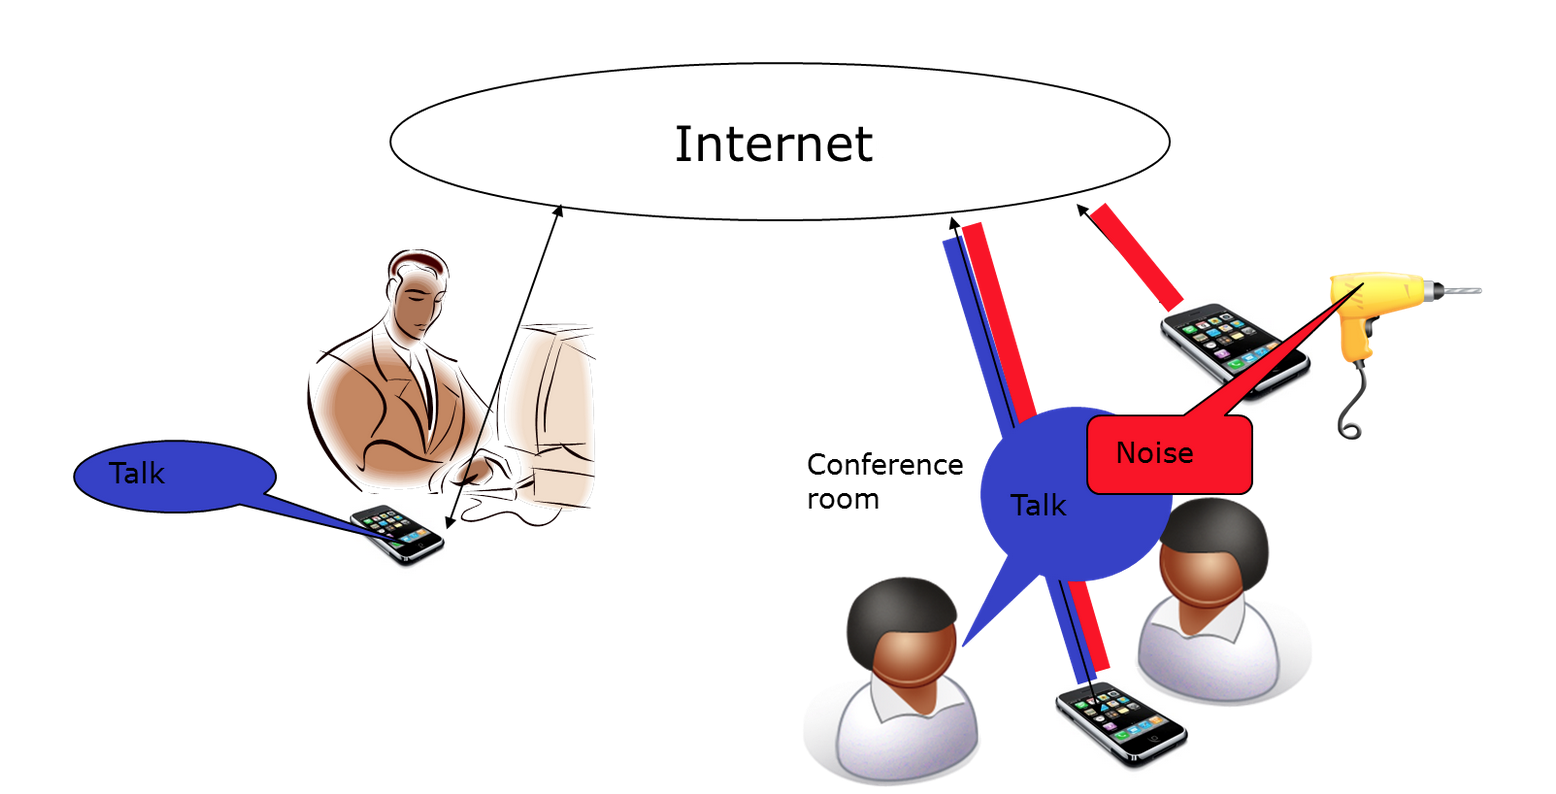
\includegraphics[width=10cm]{images/other/scenario}
		\label{scenario}
		\end{figure}

% Author and supervisor
\begin{minipage}{0.4\textwidth}
\begin{flushleft}
\emph{Authors:}\\
Animesh DAS \\ Jonas SEDIN \\ Mohammad ABDULLA \\ Thomas GAUDY \\ Xavier BUSH
\end{flushleft}
\end{minipage}
~
\begin{minipage}{0.4\textwidth}
\begin{flushright}
\emph{Advisor:}\\
Per ZETTERBERG
\end{flushright}
\end{minipage}

\vfill

% Bottom of the page
{\large Spring 2015} \\[1cm]
\end{center}



\end{titlepage}
\restoregeometry



\pagebreak\tableofcontents
\pagebreak

\chapter{Background}

	\section{Introduction of noisy environments}
	\label{sec:intronoise}
	
It is a fact that the scenarios with phone calls involved are increasing every day. This situation implies an increase of the probability of being in a noisy scenario, specially in big cities. As a result of the discomfort that the users suffer in these noisy environments, engineering and science have worked with different approaches to solve this problem.

The diversity of noise nature and its sources lead the engineering to a big challenge: develop high performance soltions in these diverse environments. When facing noise cancellation is very important to take into account the variability that the noise may experience, as previously said. Duration of the noise sequences (from \textit{ms} to long sequences), color of the noise and stationarity are possible classifications of the noise and each classification implies different ways of treating it. Therefore, a lot of systems are using combined techniques to reach the best possible performance, which has been naturally the case of this project.

	\section{Historical Overview}
	\label{historya}
	Before presenting the proposed solutions and approaches of the project, it is needed a historical overview to understand how have the group been influenced and which have been the patterns of research.


	\section{Description of the project}
	\label{sec:introproblem}
	
	The problem proposed by the course \textit{EQ2440} has been a "Noise and echo cancellation of a teleconference". The general scenario is that the first of the two speakers of the teleconference is in a noisy environment and the clear goal is to cancel as much noise as possible in order that the second speaker could receive a cleaner speech and make the conversation more comfortable. As said in \ref{sec_intronoise}, there are different approaches to solve this problem, where several of them require the availability of pure noise recordings, in our case recorded with a third phone placed close to the noise source. To have a clearer overview of the scenario the Figure \ref{scenario2} shows an approximate scheme easy to understand.
	
	When talking about denoising a teleconference there are two factors to take into account, techniques to cancel the noise and the possibility of their implementation in a real time application. The real time application has been, as expected, a big challenge because it implies good performance in terms of cancellation with the minimum reachable delay to conserve the naturalness of the conversation.
	
		\begin{figure}[h]
		\centering
		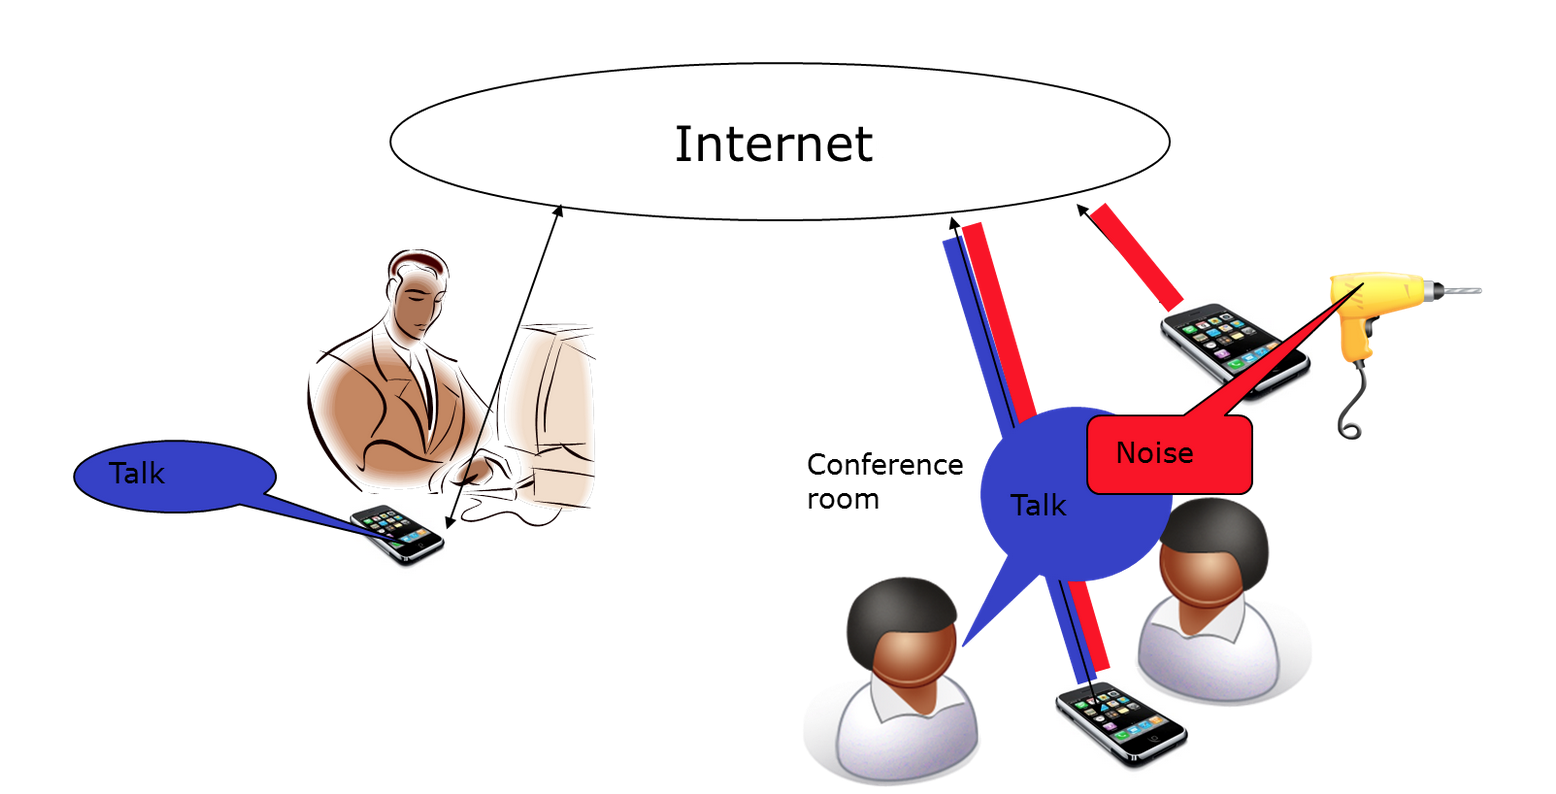
\includegraphics[width=10cm]{images/other/scenario}
		\caption{Scenario to solve}
		\label{scenario2}
		\end{figure}
	
	
	
	\section{Goal}
	As commented in \ref{sec:introproblem}, the goal is to cancel the noise contribution in the conversation between the two speakers of the teleconferences. With the purpose to simplify the scenario, it will be assumed that only one of the speakers is surrounded by noise and the main noise source is known as well.
	
	As in every engineering project, the group had to find a compromise between performance in noise cancellation and viability of implementation in real life. As it will be explained in \ref{sec:methodology}, the computational cost is a big constrain and the best performance of certain approaches (\ref{sec:theory}) introduce too much delay because of this reason. As a consequence, not always the best solution will be possible to implement in the real time version of the project.
	
	As a contrast, the personal goals of the project members are to learn form the teamwork environment, learn a research methodology, research criteria and certain skills of management that might be used in the performance of a Master Thesis (as an inmidate future) and in a research or business environment.
	
	The new knowledge acquisition is obviously another personal goal of all the team members.
	
	
	\section{Organizationn and Human Resources}
	\label{organization}

The organization of the project consists in electrical engineering students at different stages of the studies and within different specializations. In order to make the team as efficient as possible, the project has been divided in four different groups: \textit{Theory Group}, \textit{Android Group}, \textit{Multimedia Group} and \textit{Management Group}, all of them explained in detail in \ref{sec:methodology}.

The distribution of the team members has been as follows.

\begin{itemize}

\item Animesh Das
	\begin{itemize}
	\item Role: Management Group
	\item e-mail:animeshu1989@gmail.com (animeshd@kth.se)
	\item Telephone: +46 737155575
	\end{itemize}
	
\item Jonas Sedin
	\begin{itemize}
	\item Role: Theory Group \& Android Group
	\item e-mail: sedinjo@gmail.com (jonassed@kth.se)
	\item Telephone: +46 704252951
	\end{itemize}
	
\item Mohammad Abdulla
	\begin{itemize}
	\item Role: Android Group \& Multimedia Group
	\item e-mail: hamodiilatch@gmail.com (mabdulla@kth.se)
	\item Telephone: +46 737393276
	\end{itemize}
	
\item Thomas Gaudy
	\begin{itemize}
	\item Role: Android Group
	\item e-mail: gaudy.thomas@gmail.com (gaudy@kth.se)
	\item Telephone: +46 760936034
	\end{itemize}
	
\item Xavier Bush
	\begin{itemize}
	\item Role: Theory Group \& Management Group (Project Leader)
	\item e-mail: xavier.bush@gmail.com (xbush@kth.se)
	\item Telephone: +46 764141834
	\end{itemize}
	
	
\end{itemize}

The sponsor members as Project Examiner/Supervisor and Project Support are:

\begin{itemize}
\item Per Zetterberg
	\begin{itemize}
	\item Role: Project Examiner
	\item e-mail: perz@ee.kth.se
	\item Telephone: +46 8 790 77 85
	\end{itemize}
	
\item Hadi Ghauch
	\begin{itemize}
	\item Role: Group Assistant
	\item e-mail: ghauch@kth.se
	\end{itemize}
	
\item Martin Ohlsson
	\begin{itemize}
	\item Role: Android Guru
	\item e-mail: martinoh@kth.se
	\item Telephone: +46 87907818
	\end{itemize}
\end{itemize}

\chapter{Methodology}
\label{sec:methodology}

This chapter shows the methodology that the group has followed since the projecte started. On the first hand, it goes without saying that the project group has followed the \textit{Scientific Method} in the implementation of the project. On the second hand, as commented in \ref{organization}, the group has been divided in three groups explained in the following subsections.

	\section{Theory Group}

The\textit{Theory Group} had as its main goal finding solutions to cancel the present noise in the teleconference. Nevertheless, a constraint of the group has been the computational cost that the implementation have, where all the details may be found in \ref{sec:theory}.

The fact that three members of the project had recent and good background in Adaptive Signal Processing, which has been one of the chosen approaches to face the noise cancellation, made easier the making of the groups. Moreover, the \textit{Theory Group} avoided the first stage in theory research, which is the most difficult part when starting a new project.

In terms of methodology, the \textit{Theory Group} has followed next steps:

\begin{itemize}
\item Make research in suitable algorithms.
\item Record with the given mobile phones both signals: 'voice+noise' and 'noise'. 
\item Test the performance in MATLAB.
\item Check the computational cost in MATLAB.
\item Check the possibility to transfer the solutions from MATLAB to Android.
\end{itemize}

Because of the presence of Jonas Sedin in the \textit{Theory Group} and the \textit{Android Group}, it has been possible to design theory solutions think in the availability to transfer them to Android coding.\\



	\section{Android Group}
	
	This group has had two different duties:
	
	\begin{itemize}
	\item Android tasks: these tasks aimed to be an introdution to the Android programming.
	\item Noise cancellation in Android: has been the transfer from the proposed solution in the \textit{Theory Group} to Android.
	\item Real time application: optimize the code to decrease the computational cost and make possible a real time application.
	\end{itemize}
	
	In this case, even if Thomas Gaudy has not been a part of the \textit{Theory Group}, his background in Adaptive Signal Processing has helped in the implementation of the proposed solutions.
	
	\section{Multimedia Group}

This group is only formed by Mohammad Abdulla who has taken care of all the technical preparation of the presentations of the project:

\begin{itemize}
\item Video of the project: explanation of the project with real examples.
\item Power Point Presentation: power point to use in the Grand Final Presentation.
\item Bloopers Video: video containing bloopers and funny moments during the performance of the project.
\end{itemize}

	\section{Management Group}

The \textit{Management Group} has taken car of the drawing up of those tasks that were oriented to plan, follow up and present the work of the project.

The main documents are listed below:

\begin{itemize}
\item Project Plan: document that cointained a brief description of the project, time resources and planning and tasks planning.
\item Progress Report: document containing the follow up of the projects in terms of achievements and resources. It is a updated version of the Project Plan. The last Progress Report can be found in \ref{sec:appendix}.
\item Project Report: this precise document. It contains the description of all the project in all the areas.
\end{itemize}

Besides the main documents, the \textit{Management Group} has taken care of next tasks:

\begin{itemize}
\item Meetings: there has been no need to schedule meetings because of the small size of the group and the cross-group duties.
\item  Scheduling: the planning of all the tasks was designed by this group and it has been properly followed.
\end{itemize}


\section{Cross-Groups Duties}

In terms of making easier the transfer of information between groups, the makeup of the groups has followed a cross-specialization criteria. Therefore, there are team members in more than one group, and it has been possible due to the wide scope of skills that the team members have (\ref{organization}).

With this makeup, there have

\chapter{Theory}
\label{sec:theory}

The \textit{Theory Group} has been working within different scenarios but mainly has followed what is called \textit{Adaptive Signal Processing}, as it has been explained in \ref{sec:history}. Some of them have ended in good performance algorithms where only two of them have been transferred to Android and some other have not reached the wanted outcome.

In terms of goals, it has been very important for the group to reach a good noise cancellation and preserving as much as possible the voice quality.

\section{Successful Approaches}

	\subsection{LMS Algorithm}
	
		\subsubsection{Introduction}
	
	The LMS (Least Mean Square) Algorithm \cite{asp} is an adaptive filtering technique used to estimate the unwanted component in the signal that wants to be filtered and, a posteriori, subtract it to "clean" the wanted signal.
	
	To use this technique it is a needed to have both signals, the one that contains the useful information ($y(n)$) and the noisy one ($x(n)$).
	
	The process used in this technique is a recursive calculation samples by sample were $N$ previous taps of the wanted signal are used to calculate the current filter sample, used later on for the subtraction.
	
	The original problem to solve in LMS is shown in the Equation \ref{eq:lmsgeneral1}, where is clearly visible that the LMS minimizes the MSE using the instantaneous error.
	
		\begin{equation}
	\label{eq:lmsgeneral1}
		\hat{\theta}(n) = \hat{\theta}(n-1) -\frac{\mu}{2})\frac{\partial}{\partial \theta}MSE(n,\theta)\rvert_{\theta=\hat{\theta(n-1)}}
	\end{equation}
	
	Where after the appropriate calculations, the final version ready to implement in MATLAB is next:
	
	\begin{equation}
	\label{eq:lmsgeneral2}
		\hat{\theta}(n) = \hat{\theta}(n-1) + \mu Y(n)(x(n)-Y^{T}(n)\hat{\theta}(n-1))
	\end{equation}
	
	In the Equation \ref{eq:lmsgeneral2}:
	
	\begin{itemize}
	\item $\hat{\theta(n)}$: estimation of the current sample of the filter
	\item $\hat{\theta(n)}$: estimation of the previous sample of the filter
	\item $Y(n)$: vector that contains the $N$ taps used in the implementation
	\item $x(n$): sample of the unwanted signal
	\end{itemize}
	
	In terms of cost operation, LMS is very efficient thus only needs O(N) operations in each iteration. A priori, this is feasible for a real time implementation and this one of the reason that made us start with this approach.
	
	\subsubsection{Implementation \& Results}
	
	The implementation used in MATLAB is based on the one that Jonas, Thomas and Xavier have done during the course of \textit{Adaptive Signal Processing (EQ2400)}.
	
	Once all the recordings where done, the first tests of the LMS gave different performances depending on the number of previous taps used to calculate the filter.
	
	\begin{itemize}
	\item $N=1000$: very good performance with too much delay
	\item $N=100$: good performance
	\end{itemize}
	
	Another very important parameter to consider is the \textit{Step Size} $\mu$. The value of $\mu$ has a direct impact on the stability and convergence of the algorithm. The general rule of choosing the right \textit{step size} is shown in \ref{eq:stepsize}
	
	\begin{equation}
	0 < \mu <\frac{2}{\lambda_{1}} 
	\end{equation}
	
	where $\lambda_{1}$ is the maximu eigen value of $I-\mu \Sigma_{YY}$.
	
	Even though there is an upper limit for the value of $\mu$, there is not a lower limit (besides $0$). Therefore, the group followed a test-and-set empirical criteria where different $\mu$ values where tested and the value who gave the best auditive performance was the chosen. In the last case, the best performance was given by $\mu=5 \cdot 10^{-5}.$
	
	These results are reasonable: it exists a linear dependency of the performance with the number of previous samples used to calculate the current one.
	
	To show some graphic results of the performance of this algorithm, on the one hand Figure \ref{fig:lmstime100} and \ref{fig:lmstfreq100} show the time and frequency response of the filtered sequence with $N=100$ taps in comparison with the original recording. There is some audible noise reduction that in the figure can be seen in the noisy frames where there is more presence of noise in the original plot than in the filtered one. When it comes to the frequency domain, we can appreciate that there are several small peaks at low frequencies and the contribution of the peak at $f=0.6$ (where $fs=44.1$ KHz) has been slightly decreased.
	
	On the other hand,  the Figures \ref{fig:lmstime1000} and \ref{fig:lmstfreq1000} show the same comparison as before but with a filter of $N=1000$ taps. In this case the Figure \ref{fig:lmstime1000} shows that the noise has less presence. The drawback comes with a certain distortion in the audio file that can be seen in the Figure \ref{fig:lmsfreq1000} as a modification in the frequency domain with new peaks in a coarser spectral response at lower frequencies.
	
	In terms of computational time, in MATLAB the LMS with $N=100$ taps takes 2.22 seconds, while the LMS with $N=1000$ takes 3.78 seconds (increasing of a 70\%). This does not make a huge difference in MATLAB but in a real time application it might, therefore it will be treated by the \textit{Android Group}.
	
		\begin{figure}[h]
		\centering
		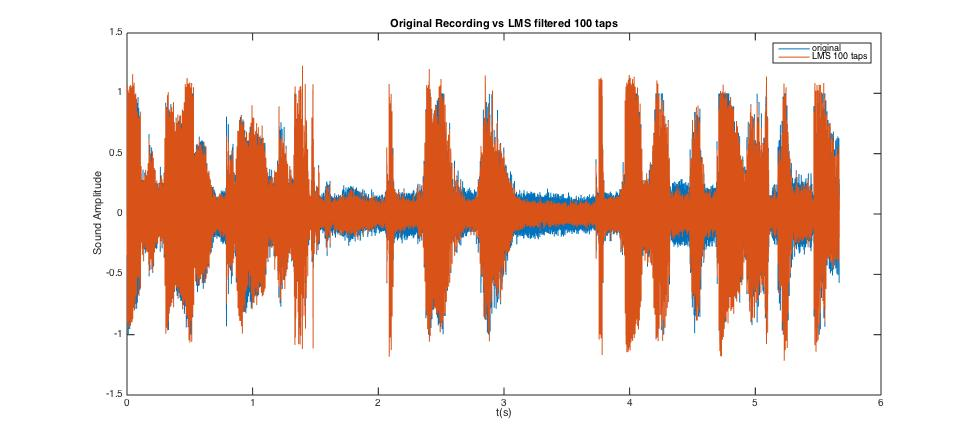
\includegraphics[width=15cm]{images/theory/lms100tapstime.jpg}
		\caption{Time Domain - LMS result with N=100}
		\label{fig:lmstime100}
		\end{figure}
		
		
		\begin{figure}[h]
		\centering
		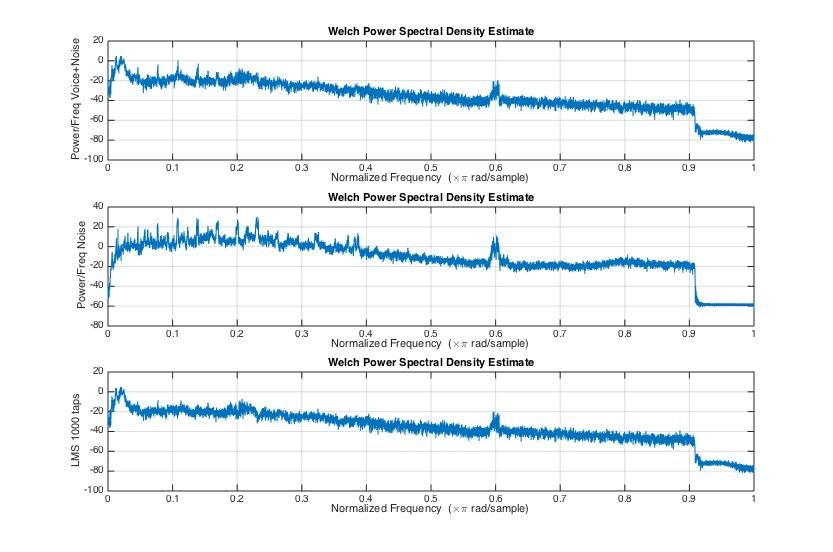
\includegraphics[width=15cm]{images/theory/lms100tapsfreq.jpg}
		\caption{Frequency Domain - LMS result with N=100}
		\label{fig:lmsfreq100}
		\end{figure}
		
		\begin{figure}[h]
		\centering
		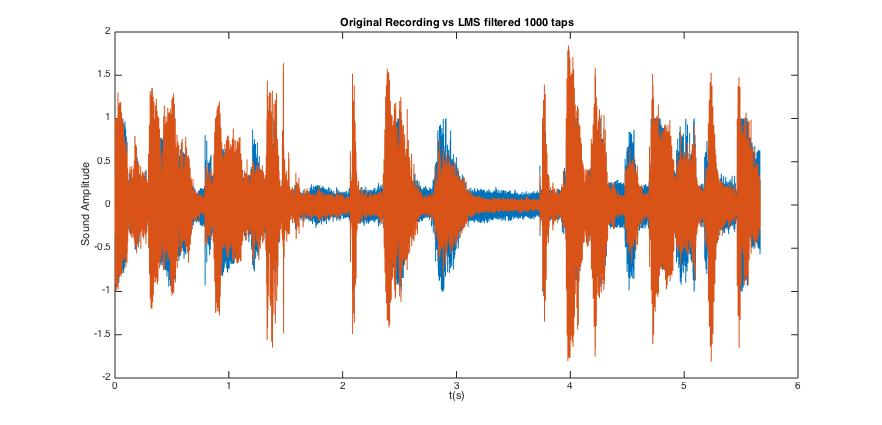
\includegraphics[width=15cm]{images/theory/lms1000tapstime.jpg}
		\caption{Time Domain - LMS result with N=1000}
		\label{fig:lmstime1000}
		\end{figure}
		
		
		\begin{figure}[h]
		\centering
		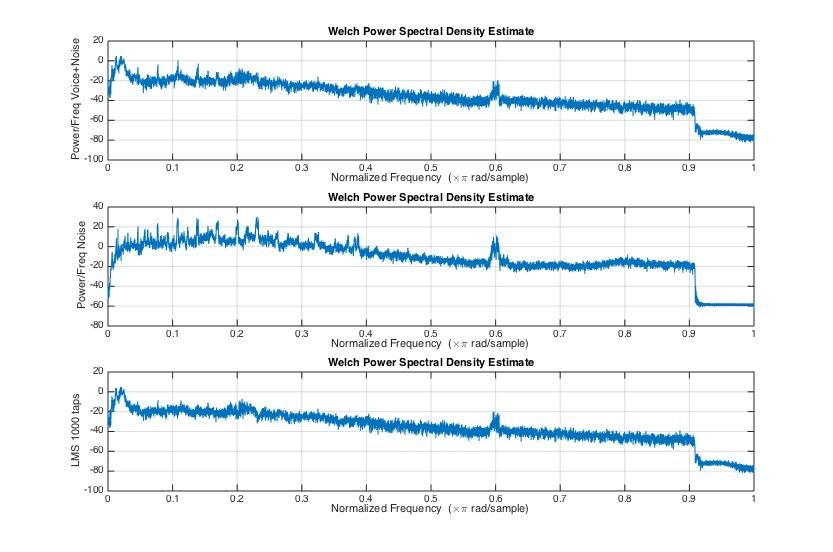
\includegraphics[width=15cm]{images/theory/lms100tapsfreq.jpg}
		\caption{Frequency Domain - LMS result with N=1000}
		\label{fig:lmsfreq1000}
		\end{figure}

	\subsection{Wiener Non-Causal Filtering}
	
	\subsubsection{Introduction}
	
	
	Wiener Filtering is another approach used in Signal Processing with many purposes and noise cancellation is one of them. Inside Wiener Filtering there are many different algorithms to use from which we have chosen Non-Causal infinite dimensional Wiener filtering \cite{asp}.
	
	One of the biggest differences between LMS Algorithm shown previously and Wiener Filtering is the number of phones involved in the filtering. Wiener Filtering does not need recording of pure noise, therefore the information of the noise will be substracted directly from the mobile of the speaker's in the noisy environment.
	
	
	\subsubsection{Implementation \& Results}
	
	\subsection{Speech Enhancement Using a-Minimum Mean- Square Error Short-Time Spectral Amplitude Estimator}


\section{Unsuccessful Approaches}

	\subsection{Kalman Filtering}
	
	
	\subsection{RLS}

\chapter{Android}

\chapter{Conclusions}

\chapter{Appendices}
\label{sec:appendix}


\bibliographystyle{plain}
\bibliography{ref}

%\include{Chapter1}			% Incluye "Chapter1.tex"


%%%%%%%% Fin del documento %%%%%%%% 
\end{document}